\documentclass[letter,11pt]{article}

\usepackage[spanish,es-nodecimaldot]{babel}
\usepackage[utf8]{inputenc}

\usepackage{lmodern}
\usepackage[T1]{fontenc}
\usepackage{textcomp}

\usepackage{framed}
\usepackage[svgnames]{xcolor}
\colorlet{shadecolor}{Gainsboro!50}

\usepackage[labelfont=bf]{caption}
\usepackage{graphicx}
\usepackage{pstricks}

\usepackage{anysize}
\marginsize{3cm}{2cm}{2cm}{3cm}

\usepackage{siunitx}
\usepackage{amsmath}
\usepackage{array}
\usepackage{csquotes}

\usepackage{fancyhdr}
\usepackage{lastpage}
\pagestyle{fancy}
\fancyhf{}
\fancyhead[LE,RO]{Laboratorio de Circuitos Eléctricos I}
\fancyfoot[CO,CE]{\thepage\ de \pageref{LastPage}}

\special{papersize=215.9mm,279.4mm}

\usepackage[
    pdfauthor={Carlos Eduardo Caballero Burgoa},%
    pdftitle={Laboratorio de Circuitos Eléctricos I},%
    pdfsubject={Métodos de análisis de circuitos},%
    colorlinks,%
    citecolor=black,%
    filecolor=black,%
    linkcolor=black,%
    urlcolor=black,
    breaklinks]{hyperref}
\usepackage{breakurl}

\newcommand{\blankpage}{
\newpage
\thispagestyle{empty}
\mbox{}
\newpage
}

\renewcommand{\arraystretch}{1.2}

\begin{document}

\begin{titlepage}
    \begin{center}
        {\Large UNIVERSIDAD MAYOR DE SAN SIMÓN}\\
        \vspace*{0.15cm}
        {\large FACULTAD DE CIENCIAS Y TECNOLOGÍA}\\
        \vspace*{0.10cm}
        DEPARTAMENTO DE ELÉCTRICA-ELECTRÓNICA\\
        \vspace*{3.0cm}
        {\Large \textbf{LABORATORIO DE CIRCUITOS ELÉCTRICOS I}}\\
        \vspace*{0.3cm}
        {\Large \textbf{INFORME No. 3}}\\
        \vspace*{3.5cm}
        {\Large \textbf{MÉTODOS DE ANÁLISIS DE CIRCUITOS}}\\
    \end{center}

    \vspace*{6.4cm}
    \leftskip=7.95cm
    \noindent
    \textbf{Estudiante:}\\
    Caballero Burgoa, Carlos Eduardo.\\
    \newline
    \textbf{Carrera:}\\
    Ing. Electromecánica.\\
    \newline
    \textbf{Docente:}\\
    Ing. Marco Antonio Vallejo Camacho.\\
    \newline
    \textbf{Grupo:} 3E.\\
    \textbf{Fecha de entrega:} 27 de Abril del 2024.\\
\end{titlepage}

\section{Cálculos previos}

\begin{figure}[!h]
\centering
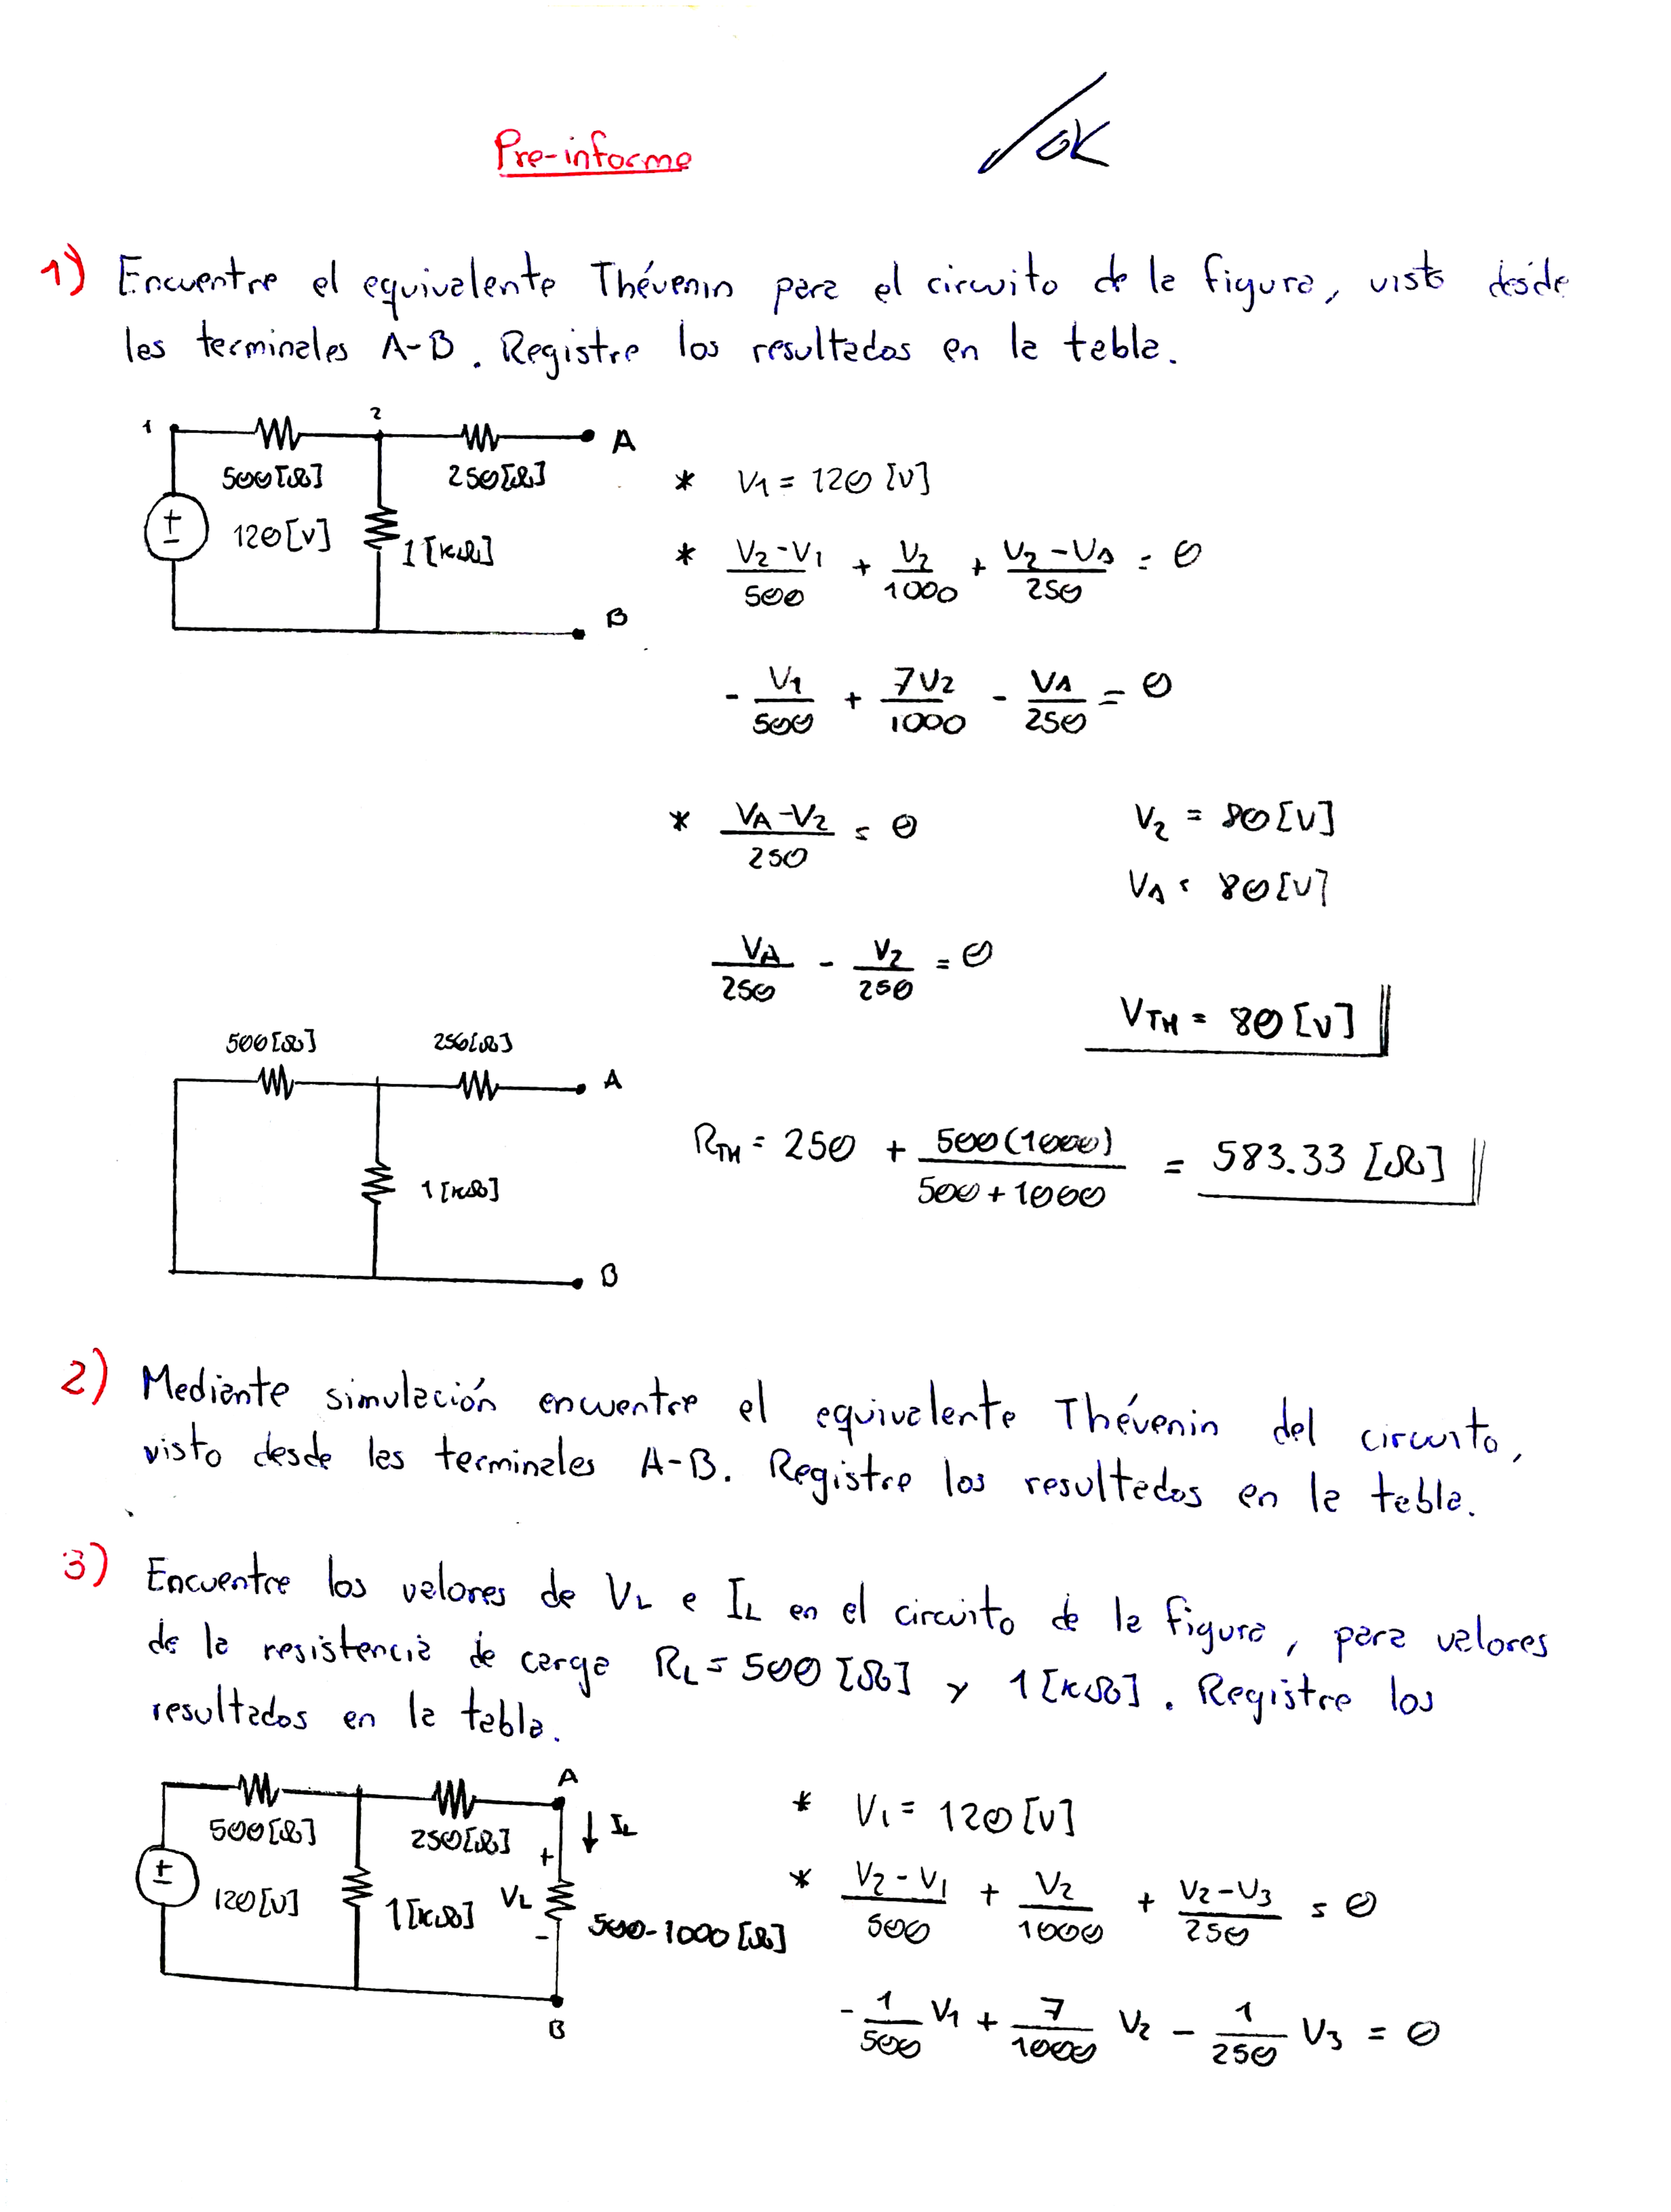
\includegraphics[scale=0.183]{resources/preinforme1.eps}
\end{figure}

\begin{figure}[!h]
\centering
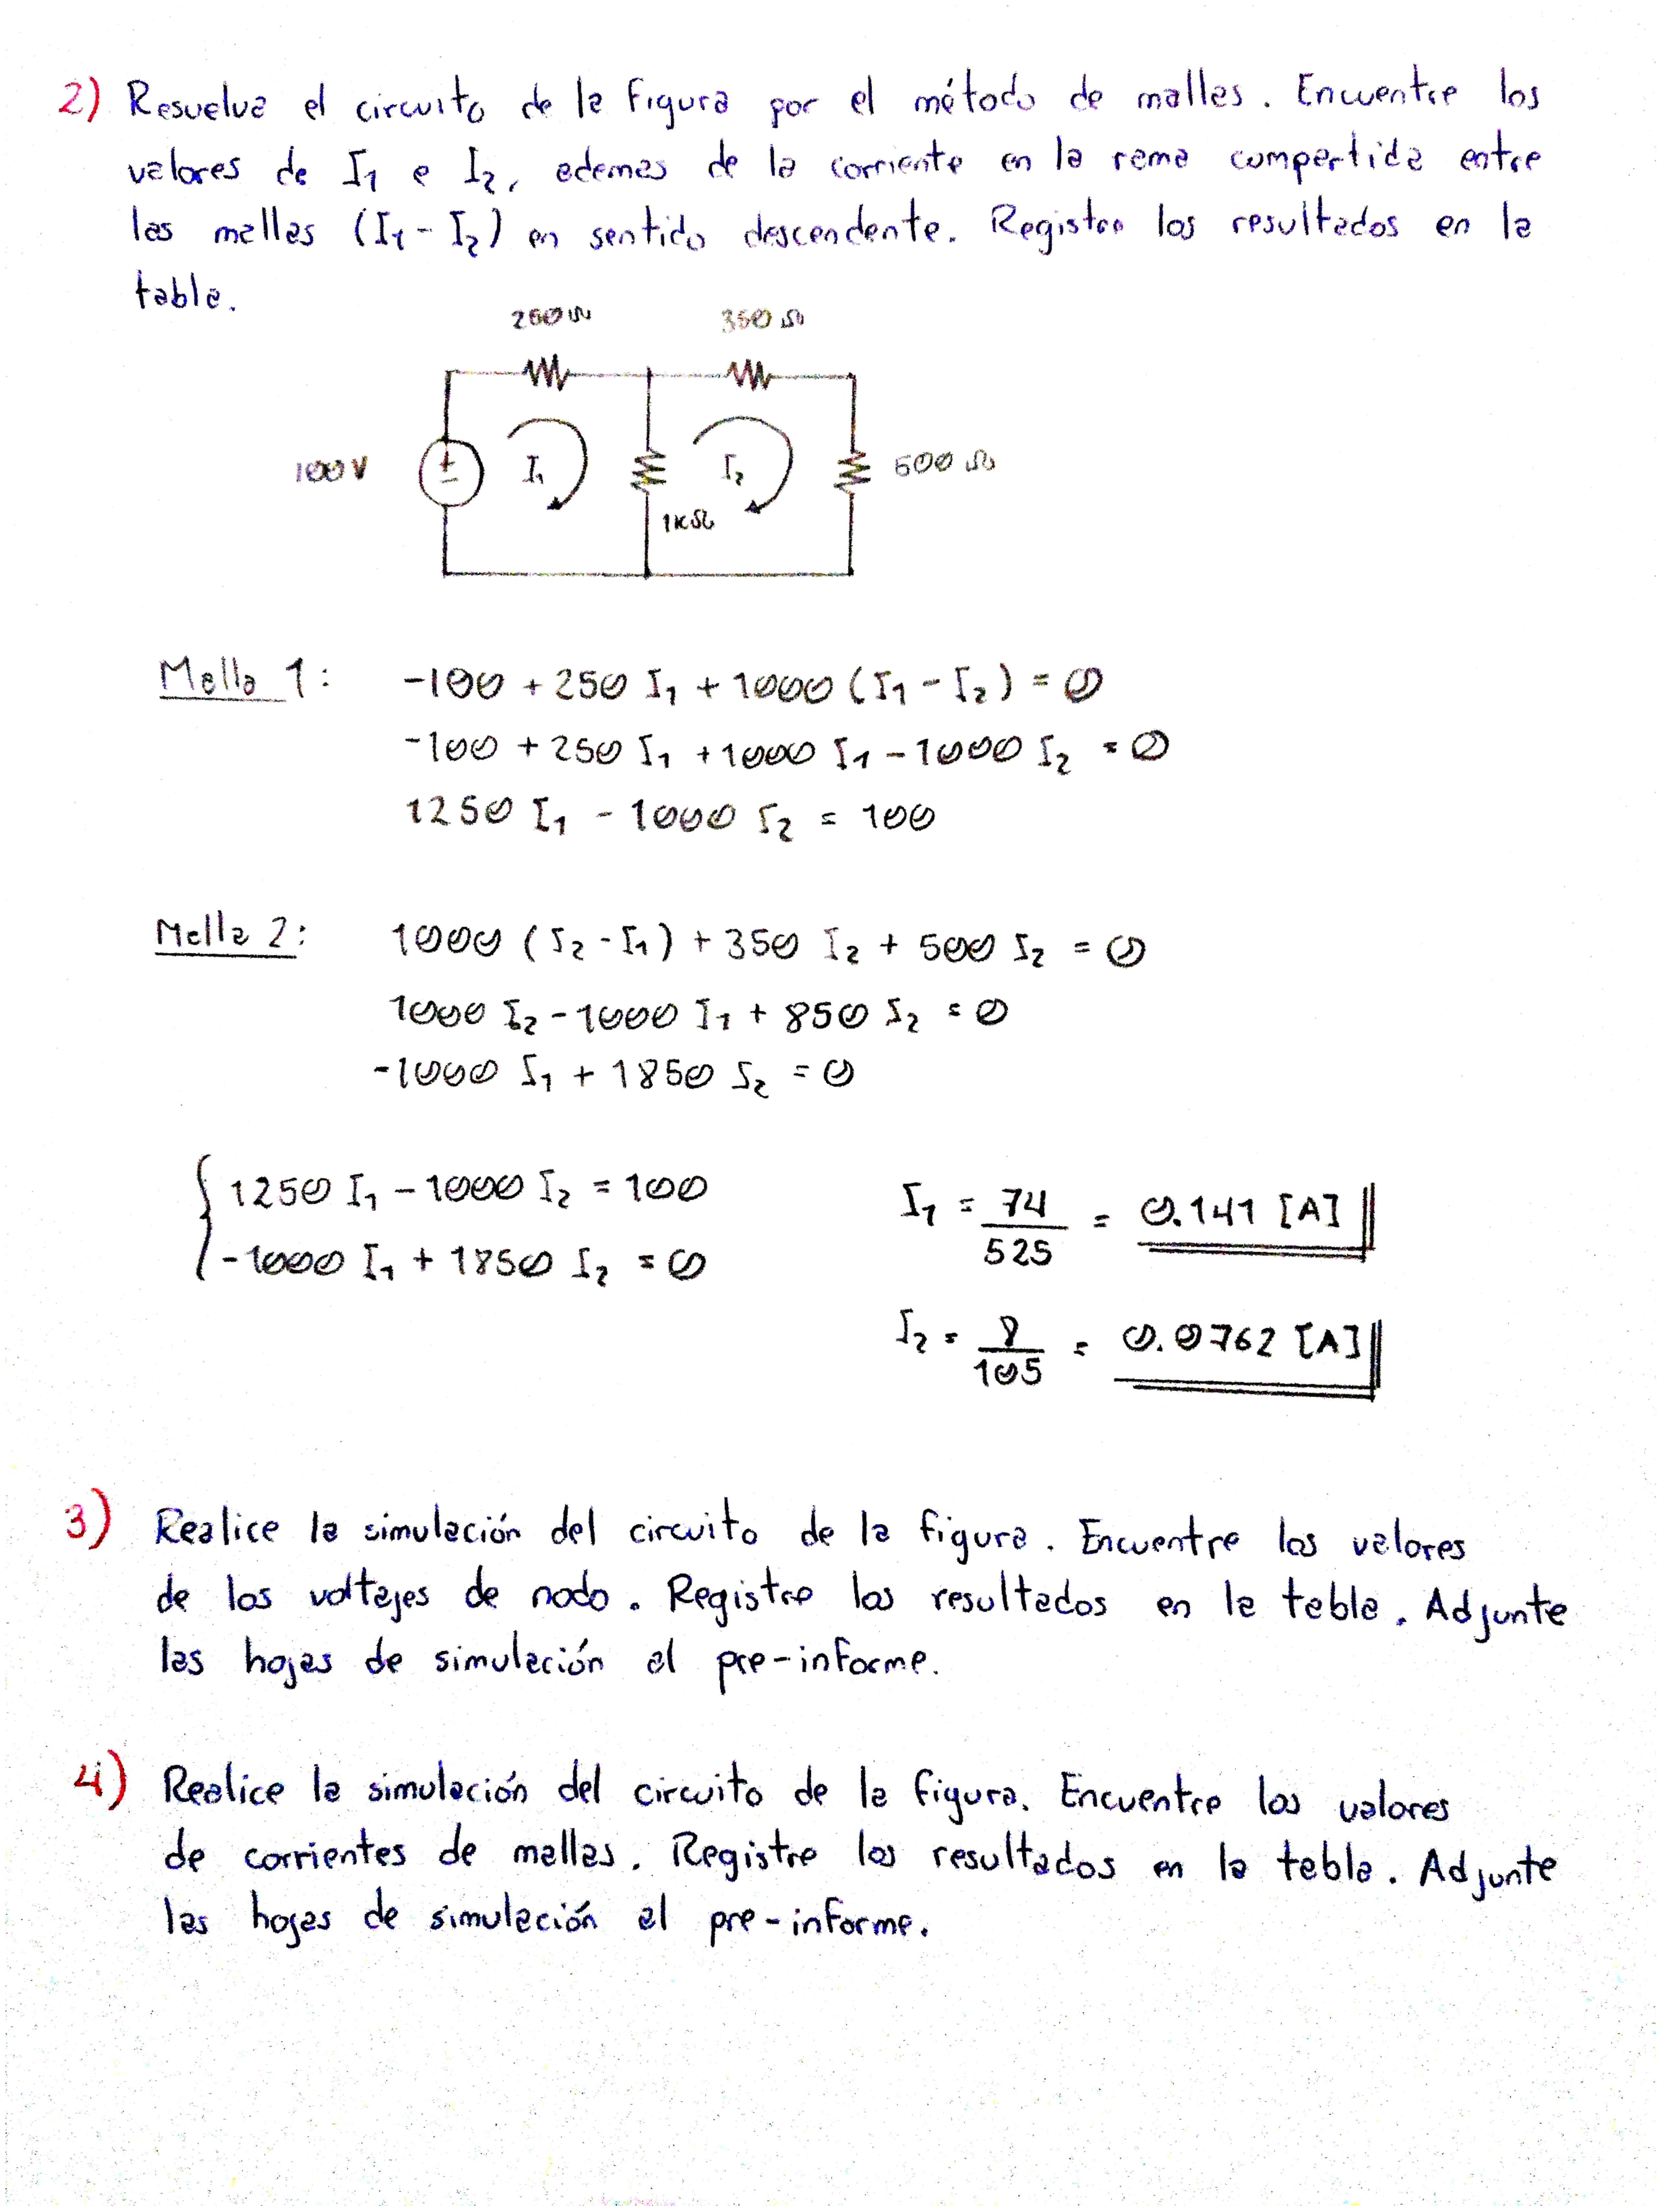
\includegraphics[scale=0.183]{resources/preinforme2.eps}
\end{figure}

\section{Simulación}
Se utilizó el software \emph{Quite Universal Circuit Simulator.} para simular
los circuitos, estos pueden verse en la figura (\ref{simulacion1}) y
(\ref{simulacion2}).
\\
\vspace{1.5cm}

\begin{figure}[!h]
\centering
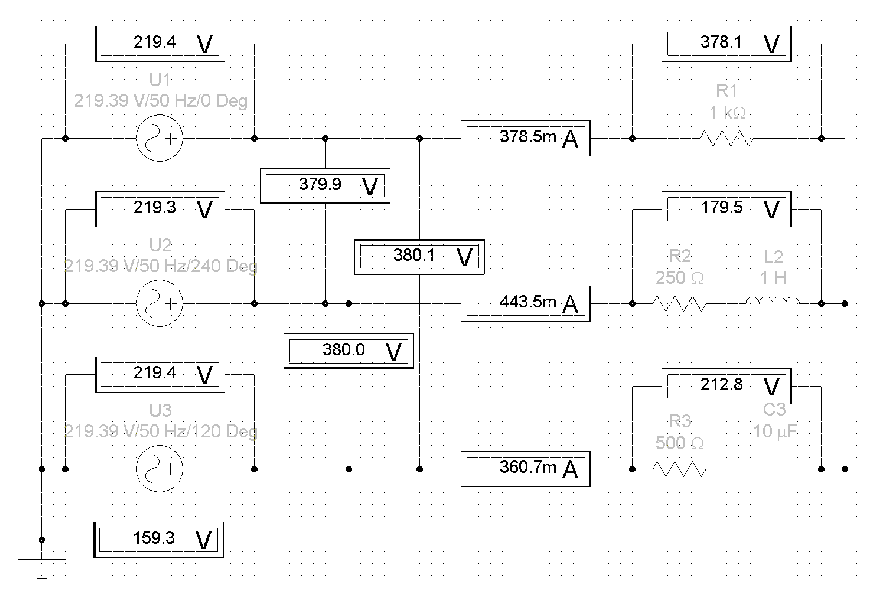
\includegraphics[scale=0.75]{simulation/practica3.1.eps}
\caption{Simulación para el método de los voltajes de nodos.}
\label{simulacion1}
\end{figure}

\newpage

\begin{figure}[!h]
\centering
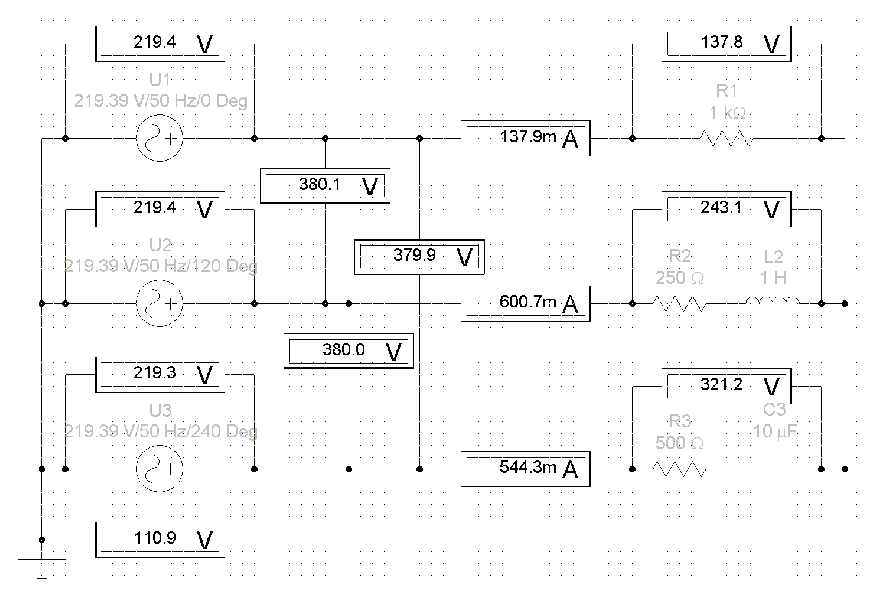
\includegraphics[scale=0.88]{simulation/practica3.2.eps}
\caption{Simulación para el método de las corrientes de mallas.}
\label{simulacion2}
\end{figure}

\section{Tablas y mediciones}
En la figura (\ref{tablas}), se adjunta la hoja de resultados provista en la
guía de laboratorio, rellenada con la información teórica, simulada y las
mediciones realizadas en laboratorio.

\begin{figure}[!h]
\centering
\includegraphics[scale=0.18]{resources/preinforme3.eps}
\caption{Tabla de resultados.}
\label{tablas}
\end{figure}

\newpage

\section{Cuestionario}

\begin{enumerate}

\item \textbf{(a) Empleando los voltajes obtenidos en el método de nodos,
determinar las corrientes indicadas en la tabla; (b) empleando las corrientes
obtenidas en el método de mallas, determinar los voltajes indicadas en la
tabla:} \\

(a)
\begin{equation*}
    I_{250[\Omega]}
        = \frac{V_a-V_b}{R_{250[\Omega]}}
        = \frac{100[V]-64.762[V]}{250[\Omega]}
        = 0.141[A]
\end{equation*}
\begin{equation*}
    I_{350[\Omega]}
        = \frac{V_b-V_c}{R_{350[\Omega]}}
        = \frac{100[V]-64.762[V]}{250[\Omega]}
        = 0.076[A]
\end{equation*}
\begin{equation*}
    I_{500[\Omega]}
        = \frac{V_c}{R_{500[\Omega]}}
        = \frac{38.095[V]}{500[\Omega]}
        = 0.076[A]
\end{equation*}
\begin{equation*}
    I_{1000[\Omega]}
        = \frac{V_b}{R_{1000[\Omega]}}
        = \frac{64.762[V]}{1000[\Omega]}
        = 0.065[A]
\end{equation*}
\begin{equation*}
    I_{100[V]} = I_{250[\Omega]} = 0.141[A]
\end{equation*}

(b)
\begin{equation*}
    V_{250[\Omega]}
        = I_1(R_{250[\Omega]})
        = (0.141[A])(250[\Omega])
        = 35.25[V]
\end{equation*}
\begin{equation*}
    V_{350[\Omega]}
        = I_2(R_{350[\Omega]})
        = (0.076[A])(350[\Omega])
        = 26.6[V]
\end{equation*}
\begin{equation*}
    V_{500[\Omega]}
        = I_2(R_{500[\Omega]})
        = (0.076[A])(500[\Omega])
        = 38[V]
\end{equation*}
\begin{equation*}
    V_{1000[\Omega]}
        = (I_1-I_2)(R_{1000[\Omega]})
        = (0.141[A]-0.076[A])(1000[\Omega])
        = 65[V]
\end{equation*}

\begin{center}
\begin{tabular}{|c|
    >{\centering}m{4.04cm}<{\centering}|
    >{\centering}m{4.04cm}<{\centering}|}
    \hline
    & 
    \textbf{Voltajes} &
    \textbf{Corrientes} \tabularnewline \hline
    \textbf{Fuente} & $100[V]$ & $0.141[A]$ \tabularnewline \hline
    $250[\Omega]$ & $V_{250[\Omega]} = 35.25[V]$ & $I_{250[\Omega]} = 0.141[A]$ \tabularnewline \hline
    $350[\Omega]$ & $V_{350[\Omega]} = 26.6[V]$ & $I_{350[\Omega]} = 0.076[A]$ \tabularnewline \hline
    $500[\Omega]$ & $V_{500[\Omega]} = 38[V]$ & $I_{500[\Omega]} = 0.076[A]$ \tabularnewline \hline
    $ 1[k\Omega]$ & $V_{ 1[k\Omega]} = 65[V]$ & $I_{ 1[k\Omega]} = 0.141[A]$ \tabularnewline \hline
\end{tabular}
\end{center}

\item \textbf{Empleando el método de análisis mas adecuado, encuentre el valor
de la corriente $I_z$ en el circuito de la figura. Considere $\beta$ como una
constante.}\\

\begin{figure}[!h]
\centering
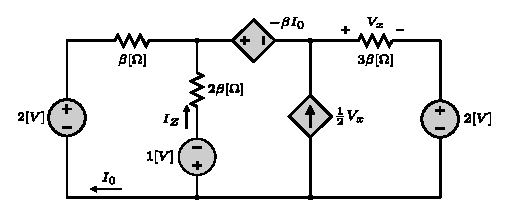
\includegraphics[width=0.75\textwidth]{resources/figura1.eps}
\end{figure}

Utilizando el método de corrientes de malla, se plantea el siguiente sistema de
ecuaciones:

\begin{equation*}
    \begin{bmatrix}
        \beta + 2\beta & -2\beta & 0 \\
        -2\beta & 2\beta & 0 \\
        0 & 0 & 3\beta
    \end{bmatrix}
    \begin{bmatrix}
        i_1 \\
        i_2 \\
        i_3
    \end{bmatrix}
    =
    \begin{bmatrix}
        1 + 2 \\
        -(-\beta\,I_0) - \frac{1}{2}\,V_x + 1 \\
        -2 + \frac{1}{2}\,V_x
    \end{bmatrix}
\end{equation*}
\begin{equation*}
    \begin{bmatrix}
        3\beta & -2\beta & 0 \\
        -2\beta & 2\beta & 0 \\
        0 & 0 & 3\beta
    \end{bmatrix}
    \begin{bmatrix}
        i_1 \\
        i_2 \\
        i_3
    \end{bmatrix}
    =
    \begin{bmatrix}
        3 \\
        \beta\,I_0 - \frac{1}{2}\,V_x + 1 \\
        \frac{1}{2}\,V_x - 2
    \end{bmatrix}
\end{equation*}

Se calcula la matriz inversa por el método de eliminación de \emph{Gauss}-\emph{Jordan}:
\begin{equation*}
    \left[
    \begin{array}{ccc|ccc}
        3\beta & -2\beta & 0 & 1 & 0 & 0 \\
        -2\beta & 2\beta & 0 & 0 & 1 & 0 \\
        0 & 0 & 3\beta & 0 & 0 & 1
    \end{array}
    \right]
    \begin{array}{c}
        \times 2 \\
        \times 3 \\
        \times 1
    \end{array}
    =
    \left[
    \begin{array}{ccc|ccc}
        6\beta & -4\beta & 0 & 2 & 0 & 0 \\
        -6\beta & 6\beta & 0 & 0 & 3 & 0 \\
        0 & 0 & 3\beta & 0 & 0 & 1
    \end{array}
    \right]
\end{equation*}
\begin{equation*}
    \left[
    \begin{array}{ccc|ccc}
        3\beta & -2\beta & 0 & 1 & 0 & 0 \\
        0 & 2\beta & 0 & 2 & 3 & 0 \\
        0 & 0 & 3\beta & 0 & 0 & 1
    \end{array}
    \right]
    \begin{array}{c}
        \times 1 \\
        \times 1 \\
        \times 1
    \end{array}
    =
    \left[
    \begin{array}{ccc|ccc}
        3\beta & -2\beta & 0 & 1 & 0 & 0 \\
        0 & 2\beta & 0 & 2 & 3 & 0 \\
        0 & 0 & 3\beta & 0 & 0 & 1
    \end{array}
    \right]
\end{equation*}
\begin{equation*}
    \left[
    \begin{array}{ccc|ccc}
        3\beta & 0 & 0 & 3 & 3 & 0 \\
        0 & 2\beta & 0 & 2 & 3 & 0 \\
        0 & 0 & 3\beta & 0 & 0 & 1
    \end{array}
    \right]
    \begin{array}{c}
        / 3\beta \\
        / 2\beta \\
        / 3\beta
    \end{array}
    =
    \left[
    \begin{array}{ccc|ccc}
        1 & 0 & 0 & \frac{1}{\beta} & \frac{1}{\beta} & 0 \\
        0 & 1 & 0 & \frac{1}{\beta} & \frac{3}{2\beta} & 0 \\
        0 & 0 & 1 & 0 & 0 & \frac{1}{3\beta}
    \end{array}
    \right]
\end{equation*}

Se calculan las corrientes de cada malla:
\begin{equation*}
    \begin{bmatrix}
        i_1 \\
        i_2 \\
        i_3
    \end{bmatrix}
    =
    \begin{bmatrix}
        \frac{1}{\beta} & \frac{1}{\beta} & 0 \\
        \frac{1}{\beta} & \frac{3}{2\beta} & 0 \\
        0 & 0 & \frac{1}{3\beta}
    \end{bmatrix}
    \begin{bmatrix}
        3 \\
        \beta\,I_0 - \frac{1}{2}\,V_x + 1 \\
        \frac{1}{2}\,V_x - 2
    \end{bmatrix}
\end{equation*}

\begin{equation*}
    \begin{split}
        i_1
            &= \frac{3}{\beta} + \frac{1}{\beta} (\beta\,I_0 - \frac{1}{2}\,V_x + 1) \\
            &= \frac{3}{\beta} + I_0 - \frac{V_x}{2\beta} + \frac{1}{\beta} \\
            &= I_0 - \frac{V_x}{2\beta} + \frac{4}{\beta}
    \end{split}
\end{equation*}

\begin{equation*}
    \begin{split}
        i_2
            &= \frac{3}{\beta} + \frac{3}{2\beta} (\beta\,I_0 - \frac{1}{2}\,V_x + 1) \\
            &= \frac{3}{\beta} + \frac{3\,I_0}{2} - \frac{3\,V_x}{4\beta} + \frac{3}{2\beta} \\
            &= \frac{3\,I_0}{2} - \frac{3\,V_x}{4\beta} + \frac{9}{2\beta} 
    \end{split}
\end{equation*}

\begin{equation*}
    \begin{split}
        i_3
            &= \frac{1}{3\beta}(\frac{1}{2}\,V_x - 2) \\
            &= \frac{V_x}{6\beta} - \frac{2}{3\beta}
    \end{split}
\end{equation*}

Por tanto $i_z$ es:
\begin{equation*}
    \begin{split}
        i_z
            &= -i_1 + i_2 \\
            &= -I_0 + \frac{V_x}{2\beta} - \frac{4}{\beta} + \frac{3\,I_0}{2} - \frac{3\,V_x}{4\beta} + \frac{9}{2\beta} \\
            &= \left(\frac{1}{2}I_0 + \frac{5\,V_x}{4\beta} + \frac{1}{2\beta}\right) [A]
    \end{split}
\end{equation*}

\end{enumerate}

\section{Conclusiones}
Se demostró que tanto el método de las corrientes de mallas, como el método de
los voltajes de nodos, son herramientas útiles a la hora de resolver circuitos
mas complejos.

Las mediciones realizadas en laboratorio presentaron cierta discrepancias con
los valores teóricos, esto se debió a la extrema sensibilidad en la resistencia
variable provista.

\end{document}

